\chapter{Laju Reaksi}\label{ch:g12:reaction-rates}

Sebotol susu yang dibiarkan di meja dapur menjadi asam dalam satu atau
dua hari; di dalam lemari es, susu itu tahan lebih dari seminggu.
Kembang api \omterm{def:g4:what-a-fire-needs:burning}{terbakar} dalam sepersekian detik, sedangkan patung batu
kapur di taman kota lapuk selama berabad-abad. \omterm{def:g8:balanced-equations:equation}{Persamaan setara} dan
\omterm{def:g10:reaction-progress-table:extent}{tabel kemajuan} memberi tahu apa yang dihasilkan sebuah reaksi dan berapa
banyak; keduanya tidak mengatakan apa pun tentang seberapa cepat. Bab
ini mengukur kecepatan reaksi, menemukan apa yang mengendalikannya, dan
menguraikan cara paling sederhana sebuah reaksi melambat seiring
berjalannya.

\begin{recall}
Konsentrasi larutan (\cref{ch:g10:concentration-and-dilution}) dan
\omterm{def:g10:reaction-progress-table:extent}{kemajuan reaksi} (\cref{ch:g10:reaction-progress-table}). \omterm{def:g11:absorbance:absorbance}{Absorbans}
larutan encer sebanding dengan konsentrasi spesies yang berwarna
(\cref{ch:g11:absorbance}). \omterm{def:g11:titration:titration}{Titrasi} mengukur jumlah sebuah spesies
(\cref{ch:g11:titration}).
\end{recall}

\begin{omfigure}
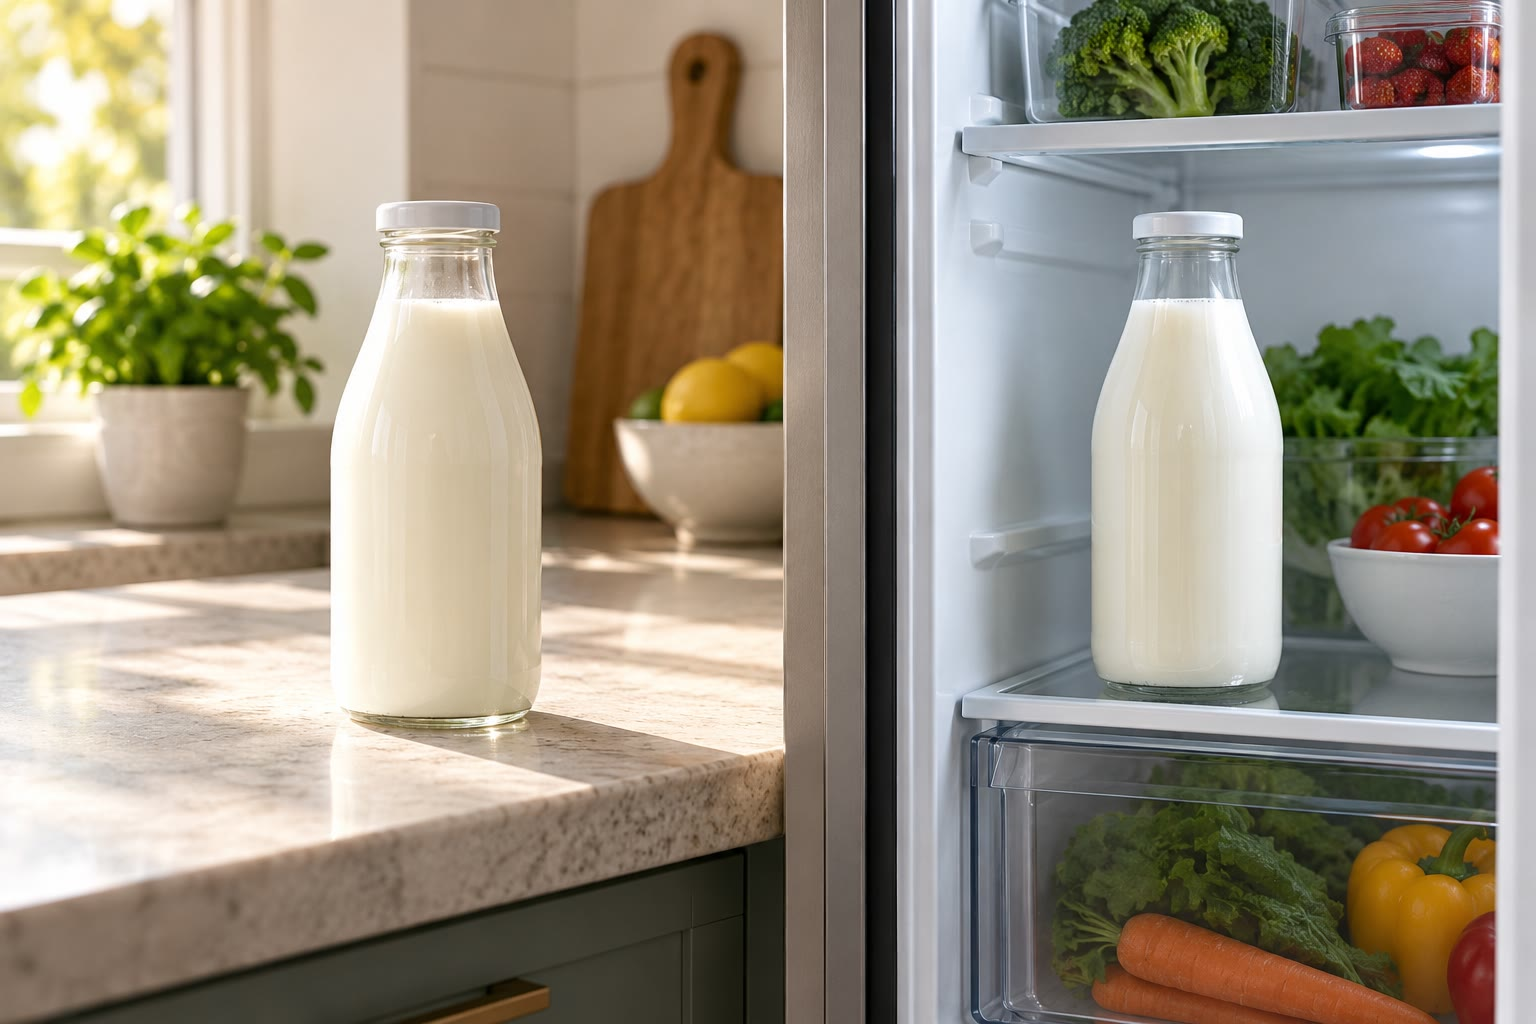
\includegraphics[width=0.48\linewidth]{images/book1/ai/g12-milk-counter-fridge.jpg}

{\small Susu yang sama, di meja dapur dan di lemari es: reaksi-reaksi
yang membuatnya asam lebih lambat dalam suhu dingin.}
\end{omfigure}

\section{Mengikuti reaksi dari waktu ke waktu}

Sebagian reaksi selesai begitu \omterm{def:g7:chemical-reactions:reactant}{pereaksinya} bertemu: pengendapan perak
klorida, reaksi asam dengan basa. Reaksi lain memerlukan beberapa
menit, beberapa jam, atau bertahun-tahun. Untuk mempelajari reaksi yang
lambat, ahli kimia mengukur konsentrasi sebuah \omterm{def:g7:chemical-reactions:reactant}{pereaksi} atau produk
pada selang waktu yang teratur. Mereka dapat
\begin{itemize}
  \item mengambil sampel-sampel kecil, menghentikan reaksi dalam setiap
        sampel, lalu menitrasinya;
  \item mengukur \omterm{def:g11:absorbance:absorbance}{absorbans} larutan, jika sebuah \omterm{def:g7:chemical-reactions:reactant}{pereaksi} atau produk
        berwarna;
  \item mengukur tekanan atau volume gas yang dilepaskan, atau daya
        hantar listrik larutan yang \omterm{def:g9:ions:ion}{ion-ionnya} berubah.
\end{itemize}

\begin{definition}[Peredaman]\label{def:g12:reaction-rates:quenching}
Yang disebut \emph{peredaman}\index{peredaman} sebuah sampel adalah
menghentikan, atau sangat memperlambat, reaksi di dalamnya pada saat
sampel itu diambil, biasanya dengan mendinginkannya secara mendadak dan
mengencerkannya, sehingga komposisinya dapat diukur dengan leluasa.
\end{definition}

\begin{inthelab}[Meredam sampel]
Setiap lima menit, \qty{10.0}{mL} \omterm{def:g6:pure-substances-and-mixtures:mixture}{campuran} reaksi diambil dengan pipet
dan dituangkan ke dalam gelas kimia berisi sekitar \qty{40}{mL} air es.
Setelah diencerkan lima kali dan didinginkan sampai mendekati
\qty{0}{\celsius}, reaksinya menjadi begitu lambat sehingga dapat
dianggap berhenti; sampel itu lalu dititrasi. Waktu sampel adalah saat
sampel itu dituangkan ke dalam air es, bukan saat \omterm{def:g11:titration:titration}{titrasinya}.
\end{inthelab}

\begin{omfigure}
\begin{tikzpicture}[font=\small, scale=0.8]
  \pic[transform shape] at (0,0) {erlenmeyer={0.4}{orange!25}};
  \node[anchor=north, align=center] at (0,-0.15) {campuran\\ reaksi};
  \pic[transform shape, rotate=-35] at (1.4,1.2) {pipette={0.6}{orange!25}};
  \draw[omProp, very thick, -{Stealth}] (1.6,0.8) -- (2.9,0.8);
  \node[anchor=south] at (2.25,0.85) {\qty{10.0}{mL}};
  \pic[transform shape] at (4,0) {beaker={0.55}{cyan!12}};
  \foreach \p in {(3.6,0.4),(4.2,0.6),(3.9,0.85),(4.4,0.3)}
    \draw[black!30, fill=white] \p ++(-0.1,-0.08) rectangle ++(0.2,0.16);
  \node[anchor=north, align=center] at (4,-0.15) {air es:\\ reaksi berhenti};
  \draw[omProp, very thick, -{Stealth}] (5.1,0.8) -- (6.4,0.8);
  \pic[transform shape] at (7.5,0) {erlenmeyer={0.35}{orange!12}};
  \pic[transform shape] at (7.5,2.75) {burette={0.7}{violet!45}};
  \node[anchor=north, align=center] at (7.5,-0.15) {titrasi\\ sampel};
\end{tikzpicture}

{\small Mengikuti reaksi dengan pengambilan sampel: ambil sampel, redam,
lalu ukur dengan leluasa.}
\end{omfigure}

\section{Faktor kinetik}

\begin{definition}[Faktor kinetik]\label{def:g12:reaction-rates:kinetic-factor}
Yang disebut \emph{faktor kinetik}\index{faktor kinetik} adalah besaran
yang mengubah kecepatan sebuah reaksi tanpa mengubah apa yang dihasilkan
reaksi itu: suhu, konsentrasi \omterm{def:g7:chemical-reactions:reactant}{pereaksi}, luas bidang sentuh antara
\omterm{def:g7:chemical-reactions:reactant}{pereaksi-pereaksi} yang berada dalam fase berbeda, dan keberadaan katalis
(bab berikutnya).
\end{definition}

\begin{proposition}[Lebih panas, lebih pekat, lebih halus: lebih cepat]\label{prop:g12:reaction-rates:factors}
Pada umumnya sebuah reaksi lebih cepat jika suhunya lebih tinggi, jika
\omterm{def:g7:chemical-reactions:reactant}{pereaksinya} lebih pekat, dan, untuk \omterm{def:g7:chemical-reactions:reactant}{pereaksi} padat, jika \omterm{def:g7:chemical-reactions:reactant}{pereaksi} itu
lebih halus.
\end{proposition}

\begin{proof}
Diterima tanpa bukti, dengan sebuah gambaran: partikel-partikel yang
bereaksi harus bertemu, dan bertemu cukup keras. Memekatkannya membuat
pertemuan lebih sering; menghaluskan padatan memberikan permukaan yang
lebih luas untuk bertemu; memanaskan membuat partikel bergerak lebih
cepat, sehingga lebih sering bertemu dan, terutama, lebih banyak
pertemuan yang cukup berenergi untuk memutus ikatan.
\end{proof}

\begin{example}[Tiga kasus sehari-hari]\label{ex:g12:reaction-rates:everyday}
Makanan lebih tahan lama di lemari es dan jauh lebih lama lagi di
pembeku: reaksi-reaksi yang merusaknya melambat dalam suhu dingin. Debu
tepung halus di \omterm{def:g4:air-a-mixture-of-gases:air}{udara} sebuah penggilingan dapat meledak, sedangkan
sekarung tepung hanya membara: reaksinya sama, luas bidang sentuhnya
sangat besar. Tablet yang berbuih dalam air \omterm{def:g2:mixing-and-dissolving:dissolve}{larut} lebih cepat jika
digerus terlebih dahulu.
\end{example}

\begin{omfigure}
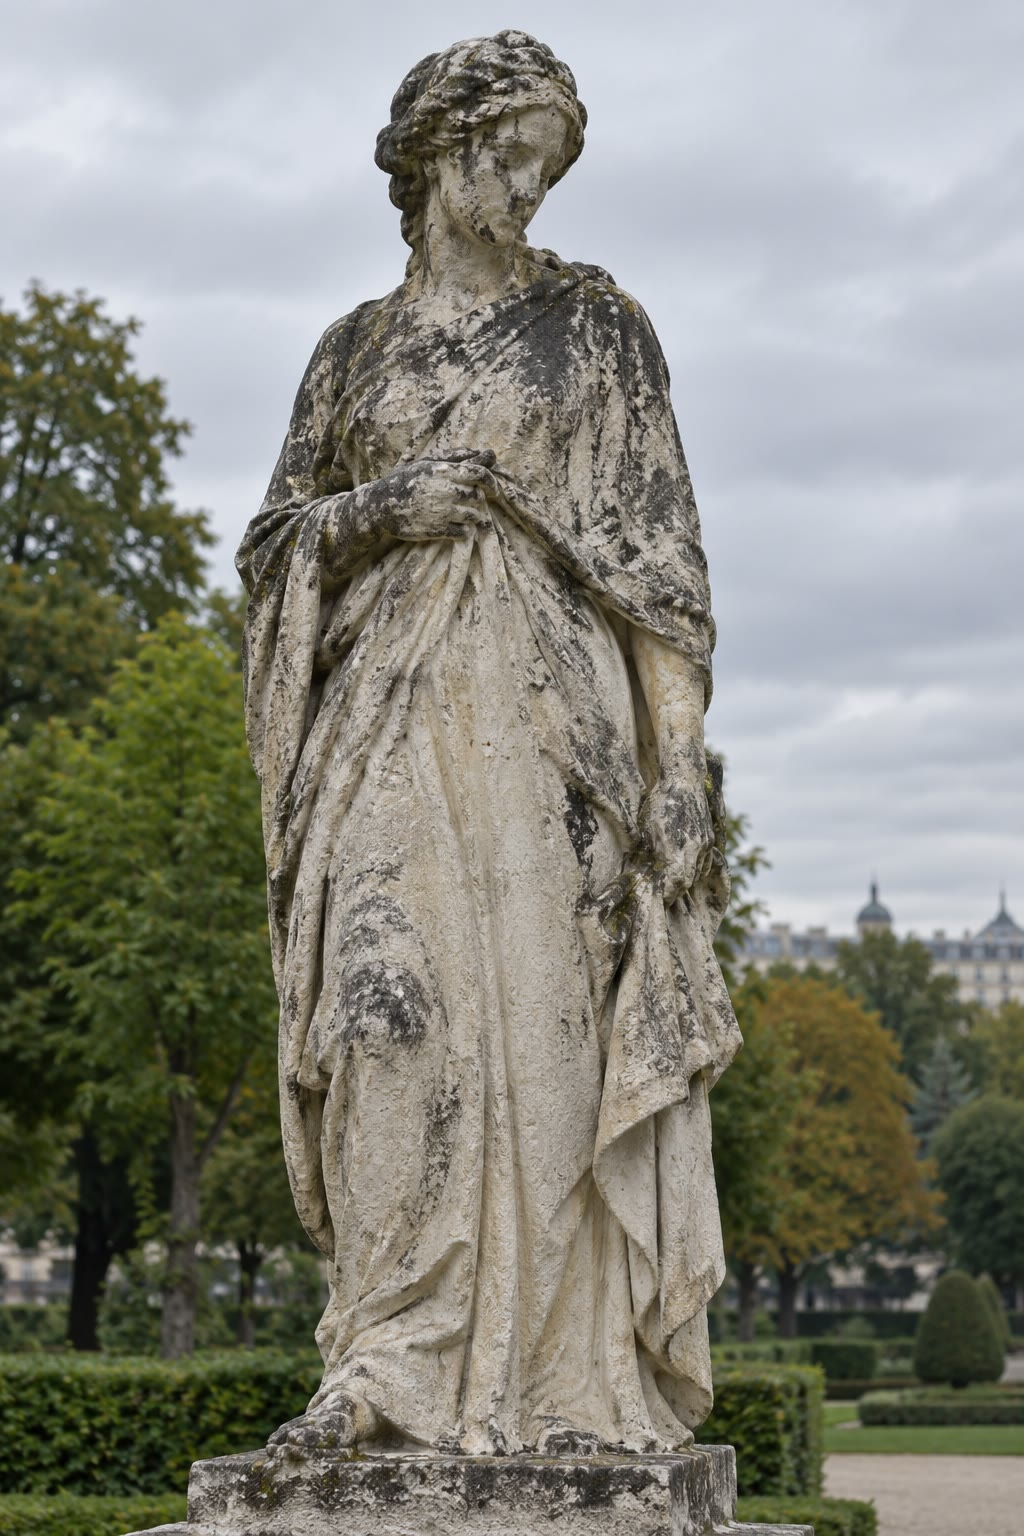
\includegraphics[width=0.42\linewidth,height=6cm,keepaspectratio]{images/book1/ai/g12-weathered-statue.jpg}

{\small Patung batu kapur yang lapuk oleh hujan: sebuah reaksi yang
berlangsung berabad-abad.}
\end{omfigure}

\section{Laju penghilangan dan laju pembentukan}

\begin{definition}[Laju penghilangan, laju pembentukan]\label{def:g12:reaction-rates:rate}
Dalam larutan yang volumenya tetap, \emph{laju penghilangan}\index{laju penghilangan}
sebuah \omterm{def:g7:chemical-reactions:reactant}{pereaksi} A pada waktu $t$ adalah
\[
  v_A(t) = -\frac{d[\ce{A}]}{dt},
\]
dan \emph{laju pembentukan}\index{laju pembentukan} sebuah produk P
adalah $v_P(t) = \dfrac{d[\ce{P}]}{dt}$. Keduanya positif, dalam
\si{mol.L^{-1}.min^{-1}} (atau per detik).
\end{definition}


\begin{method}[Membaca laju dari garis singgung]\label{met:g12:reaction-rates:tangent}
\begin{enumerate}
  \item Pada kurva $[\ce{A}]$ terhadap $t$, gambarlah garis singgung
        pada waktu yang dipilih.
  \item Bacalah dua titik yang berjauhan pada garis singgung itu, lalu
        hitung kemiringannya, $\Delta[\ce{A}] / \Delta t$.
  \item \omterm{def:g12:reaction-rates:rate}{Laju penghilangan} adalah lawan dari kemiringan ini (untuk
        produk, kemiringan itu sendiri).
\end{enumerate}
\end{method}

\begin{omfigure}
\begin{tikzpicture}
\begin{axis}[width=0.8\linewidth, height=6.4cm, xmin=0, xmax=60, ymin=0,
    ymax=11, xlabel={$t$ (\si{min})}, ylabel={$[\ce{A}]$ (\si{mmol/L})},
    axis lines*=left, ymajorgrids, xmajorgrids, grid style={gray!20},
    tick label style={font=\small}, label style={font=\small},
    legend style={font=\small, at={(0.98,0.97)}, anchor=north east,
    draw=none, fill=white}, legend cell align=left]
  \addplot[very thick, omDef] table[x=t, y=A1] {figdata/out/grade-12-reaction-rates-a.dat};
  \addplot[very thick, omThm] table[x=t, y=A2] {figdata/out/grade-12-reaction-rates-a.dat};
  \addplot[thick, dashed, omProp, restrict y to domain=0:11] table[x=t, y=tangent]
    {figdata/out/grade-12-reaction-rates-a.dat};
  \legend{$k = \qty{0.050}{min^{-1}}$, $k = \qty{0.100}{min^{-1}}$ (lebih hangat),
    garis singgung pada $t = 0$}
  \addplot[densely dotted, black!60] coordinates {(0,5) (13.86,5) (13.86,0)};
  \addplot[densely dotted, black!60] coordinates {(6.93,5) (6.93,0)};
  \node[font=\small, anchor=south west] at (axis cs:14.6,5.4) {$t_{1/2} = \qty{13.9}{min}$};
  \node[font=\small, anchor=south east] at (axis cs:6.7,0.2) {\qty{6.9}{min}};
\end{axis}
\end{tikzpicture}

{\small Konsentrasi sebuah \omterm{def:g7:chemical-reactions:reactant}{pereaksi} A terhadap waktu, untuk \omterm{def:g12:reaction-rates:first-order}{reaksi orde
satu} yang sama pada dua suhu. Garis singgung pada $t = 0$ (putus-putus)
memberikan laju awal; garis-garis titik menandai \omterm{def:g12:reaction-rates:half-life}{waktu paruhnya}.}
\end{omfigure}

\begin{example}[Laju awal]\label{ex:g12:reaction-rates:initial}
Pada kurva biru, garis singgung pada $t = 0$ berjalan dari
\qty{10.0}{mmol/L} pada $t = 0$ sampai $0$ pada $t = \qty{20}{min}$:
kemiringannya $-10.0/20 = \qty{-0.50}{mmol.L^{-1}.min^{-1}}$, jadi \omterm{def:g12:reaction-rates:rate}{laju
penghilangan} awalnya \qty{0.50}{mmol.L^{-1}.min^{-1}}. Kemudian kurvanya
melandai dan lajunya turun: reaksinya melambat seiring habisnya A.
\end{example}

\section{Reaksi orde satu}

\begin{definition}[Reaksi orde satu, tetapan laju]\label{def:g12:reaction-rates:first-order}
Sebuah reaksi disebut \emph{reaksi orde satu}\index{reaksi orde satu}
terhadap A jika \omterm{def:g12:reaction-rates:rate}{laju penghilangannya} sebanding dengan konsentrasi A pada
setiap saat:
\[
  -\frac{d[\ce{A}]}{dt} = k\,[\ce{A}] .
\]
Tetapan positif $k$, dalam \si{min^{-1}} atau \si{s^{-1}}, disebut
\emph{tetapan laju}\index{tetapan laju}; nilainya bergantung pada suhu.
\end{definition}

\begin{proposition}[Peluruhan eksponensial]\label{prop:g12:reaction-rates:exponential}
Untuk \omterm{def:g12:reaction-rates:first-order}{reaksi orde satu} dengan konsentrasi awal $[\ce{A}]_0$,
\[
  [\ce{A}](t) = [\ce{A}]_0\, e^{-kt} .
\]
\end{proposition}

\begin{proof}
Fungsi $f(t) = [\ce{A}]_0 e^{-kt}$ memiliki turunan
$f'(t) = -k [\ce{A}]_0 e^{-kt} = -k f(t)$, sehingga fungsi itu memenuhi
persamaan laju, dan $f(0) = [\ce{A}]_0$. Bahwa fungsi itu satu-satunya
fungsi semacam itu diterima di sini tanpa bukti (hal itu dibuktikan
dalam matematika, untuk persamaan $y' = ay$).
\end{proof}

\begin{method}[Menguji orde satu]\label{met:g12:reaction-rates:test}
\begin{enumerate}
  \item Dari hasil pengukuran, hitung $\ln [\ce{A}]$ (atau $\ln A$ untuk
        \omterm{def:g11:absorbance:absorbance}{absorbans} yang sebanding dengan $[\ce{A}]$) pada setiap waktu.
  \item Gambarlah grafik $\ln[\ce{A}]$ terhadap $t$: karena
        $\ln[\ce{A}] = \ln[\ce{A}]_0 - kt$, titik-titiknya terletak pada
        sebuah garis lurus jika dan hanya jika reaksinya berorde satu.
  \item Kemiringan garis itu adalah $-k$.
\end{enumerate}
\end{method}

\section{Waktu paruh}

\begin{definition}[Waktu paruh]\label{def:g12:reaction-rates:half-life}
Yang disebut \emph{waktu paruh}\index{waktu paruh} $t_{1/2}$ sebuah
reaksi adalah waktu yang diperlukan agar konsentrasi \omterm{def:g10:reaction-progress-table:limiting}{pereaksi pembatas}
turun menjadi setengah nilai awalnya.
\end{definition}

\begin{proposition}[Waktu paruh reaksi orde satu]\label{prop:g12:reaction-rates:half-life}
Untuk \omterm{def:g12:reaction-rates:first-order}{reaksi orde satu},
\[
  t_{1/2} = \frac{\ln 2}{k},
\]
berapa pun konsentrasi awalnya; setelah $n$ kali \omterm{def:g12:reaction-rates:half-life}{waktu paruh},
konsentrasinya terbagi $2^n$.
\end{proposition}

\begin{proof}
$[\ce{A}]_0 e^{-k t_{1/2}} = [\ce{A}]_0 / 2$ memberikan
$e^{-k t_{1/2}} = 1/2$, jadi $k t_{1/2} = \ln 2$. Setiap \omterm{def:g12:reaction-rates:half-life}{waktu paruh}
berikutnya mengalikan lagi konsentrasinya dengan $e^{-k t_{1/2}} = 1/2$.
\end{proof}


\begin{example}[Membaca waktu paruh]\label{ex:g12:reaction-rates:half-lives}
Untuk $k = \qty{0.050}{min^{-1}}$, $t_{1/2} = 0.693 / 0.050 =
\qty{13.9}{min}$: konsentrasinya turun dari 10.0 menjadi 5.0, lalu 2.5,
lalu \qty{1.25}{mmol/L} pada 13.9, 27.7, dan \qty{41.6}{min}. Percobaan
yang lebih hangat, dengan $k$ dua kali lebih besar, memiliki \omterm{def:g12:reaction-rates:half-life}{waktu paruh}
setengahnya, \qty{6.9}{min}, seperti yang diperlihatkan gambar.
\end{example}

\begin{remark}[Waktu paruh di tempat lain]\label{rem:g12:reaction-rates:radioactive}
Istilah yang sama dipakai dalam fisika untuk inti radioaktif, yang
jumlahnya berkurang secara eksponensial dengan cara yang sama: peluruhan
radioaktif berperilaku seperti \omterm{def:g12:reaction-rates:first-order}{reaksi orde satu}. Buku fisika
membahasnya.
\end{remark}

\begin{omfigure}
\begin{minipage}{0.49\linewidth}
\begin{tikzpicture}
\begin{axis}[width=\linewidth, height=5.4cm, xmin=0, xmax=26, ymin=0,
    ymax=0.85, xlabel={$t$ (\si{min})}, ylabel={absorbans $A$},
    axis lines*=left, ymajorgrids, grid style={gray!20},
    tick label style={font=\scriptsize}, label style={font=\small}]
  \addplot[only marks, mark=*, mark size=1.8pt, omDef] table[x=t, y=A]
    {figdata/out/grade-12-reaction-rates-b.dat};
  \addplot[thick, omProp, domain=0:26, samples=60] {0.8*exp(-0.11552*x)};
\end{axis}
\end{tikzpicture}
\end{minipage}\hfill
\begin{minipage}{0.49\linewidth}
\begin{tikzpicture}
\begin{axis}[width=\linewidth, height=5.4cm, xmin=0, xmax=26, ymin=-3.4,
    ymax=0, xlabel={$t$ (\si{min})}, ylabel={$\ln A$}, axis lines*=left,
    ymajorgrids, grid style={gray!20}, tick label style={font=\scriptsize},
    label style={font=\small}]
  \addplot[only marks, mark=*, mark size=1.8pt, omDef] table[x=t, y=lnA]
    {figdata/out/grade-12-reaction-rates-b.dat};
  \addplot[thick, omProp, domain=0:26] {-0.2231-0.11552*x};
\end{axis}
\end{tikzpicture}
\end{minipage}

{\small Memudarnya kristal violet dalam \omterm{def:g9:acids-bases-ph:acidic}{larutan basa} (data soal akhir
pekan). Kiri: \omterm{def:g11:absorbance:absorbance}{absorbansnya} turun mengikuti kurva eksponensial. Kanan:
$\ln A$ terhadap $t$ berupa garis lurus dengan kemiringan
$-\qty{0.116}{min^{-1}}$: reaksinya berorde satu terhadap zat warna.}
\end{omfigure}

\section{Latihan}

\begin{exercise}[$\star$]\label{exo:g12:reaction-rates:1}
Sebutkan \omterm{def:g12:reaction-rates:kinetic-factor}{faktor kinetik} yang berperan dalam setiap kasus: lemari es
mengawetkan makanan; gula halus \omterm{def:g2:mixing-and-dissolving:dissolve}{larut} lebih cepat daripada gula
bongkahan; asam yang lebih pekat menyerang seng lebih cepat; apel yang
dipotong lebih cepat menjadi cokelat pada musim panas.
\end{exercise}

\begin{exercise}[$\star$]\label{exo:g12:reaction-rates:2}
Bacalah \omterm{def:g12:reaction-rates:half-life}{waktu paruh} setiap percobaan pada gambar $[\ce{A}]$ terhadap
waktu. Berapa $[\ce{A}]$ pada kurva biru setelah dua kali \omterm{def:g12:reaction-rates:half-life}{waktu paruh}?
\end{exercise}

\begin{exercise}[$\star$]\label{exo:g12:reaction-rates:3}
Sebuah garis singgung pada kurva sebuah produk yang digambar pada
$t = \qty{5}{min}$ melalui $(0, \qty{1.0}{mmol/L})$ dan
$(\qty{10}{min}, \qty{5.0}{mmol/L})$. Berapa \omterm{def:g12:reaction-rates:rate}{laju pembentukan} produk
itu pada \qty{5}{min}?
\end{exercise}

\begin{exercise}[$\star$]\label{exo:g12:reaction-rates:4}
Mengapa sebuah sampel dituangkan ke dalam air es sebelum dititrasi?
Mengapa waktu sampel harus dicatat saat sampel itu dituangkan, bukan
saat dititrasi?
\end{exercise}

\begin{exercise}[$\star$]\label{exo:g12:reaction-rates:5}
Sebuah \omterm{def:g12:reaction-rates:first-order}{reaksi orde satu} memiliki \omterm{def:g12:reaction-rates:half-life}{waktu paruh} \qty{10}{min}. Berapa
bagian \omterm{def:g7:chemical-reactions:reactant}{pereaksi} yang tersisa setelah \qty{30}{min}? Setelah
\qty{1}{h}?
\end{exercise}

\begin{exercise}[$\star\star$]\label{exo:g12:reaction-rates:6}
Konsentrasi sebuah \omterm{def:g7:chemical-reactions:reactant}{pereaksi}, dalam \si{mmol/L}: 8.00 pada
\qty{0}{min}, 5.66 pada \qty{5}{min}, 4.00 pada \qty{10}{min}, 2.83
pada \qty{15}{min}, 2.00 pada \qty{20}{min}. Hitung $\ln[\ce{A}]$ pada
setiap waktu dan tunjukkan bahwa reaksinya berorde satu. Tentukan $k$
dan \omterm{def:g12:reaction-rates:half-life}{waktu paruhnya}.
\end{exercise}

\begin{exercise}[$\star\star$]\label{exo:g12:reaction-rates:7}
Sebuah \omterm{def:g12:reaction-rates:first-order}{reaksi orde satu} memiliki $t_{1/2} = \qty{25}{s}$. Hitung $k$.
\end{exercise}

\begin{exercise}[$\star\star$]\label{exo:g12:reaction-rates:8}
Untuk $[\ce{A}]_0 = \qty{0.100}{mol/L}$ dan $k = \qty{0.020}{min^{-1}}$,
hitung $[\ce{A}]$ setelah 10, 30, dan \qty{100}{min}.
\end{exercise}

\begin{exercise}[$\star\star$]\label{exo:g12:reaction-rates:9}
Pada gambar $[\ce{A}]$ terhadap waktu, perkirakan kemiringan kurva biru
pada $t = \qty{13.9}{min}$ (gambarlah garis singgung), lalu bandingkan
dengan $-k[\ce{A}]$ pada waktu itu.
\end{exercise}

\begin{exercise}[$\star\star$]\label{exo:g12:reaction-rates:10}
Iodin \ce{I2}, yang cokelat, terbentuk perlahan dalam larutan tak
berwarna. \omterm{def:g11:absorbance:absorbance}{Absorbansnya} naik dari 0 menuju 0.60. Jelaskan mengapa
\omterm{def:g11:absorbance:absorbance}{absorbans} dapat dipakai untuk mengikuti $[\ce{I2}]$, dan bagaimana \omterm{def:g12:reaction-rates:rate}{laju
pembentukan} pada suatu waktu dibaca pada kurva $A$ terhadap $t$.
\end{exercise}

\begin{exercise}[$\star\star$]\label{exo:g12:reaction-rates:11}
Dua percobaan dengan reaksi yang sama dimulai pada $[\ce{A}]_0 = 10$
dan \qty{20}{mmol/L}. Jika reaksinya berorde satu, bandingkan laju awal
dan \omterm{def:g12:reaction-rates:half-life}{waktu paruh} keduanya.
\end{exercise}

\begin{exercise}[$\star\star\star$]\label{exo:g12:reaction-rates:12}
Berapa kali \omterm{def:g12:reaction-rates:half-life}{waktu paruh} yang diperlukan \omterm{def:g12:reaction-rates:first-order}{reaksi orde satu} agar
\omterm{def:g7:chemical-reactions:reactant}{pereaksinya} tinggal \qty{1}{\percent}? \qty{0.1}{\percent}? Berikan
rumus umum waktu yang diperlukan untuk turun menjadi pecahan $f$.
\end{exercise}

\begin{exercise}[$\star\star\star$]\label{exo:g12:reaction-rates:13}
Sebuah reaksi memiliki $k = \qty{0.050}{min^{-1}}$ pada
\qty{20}{\celsius} dan $k = \qty{0.100}{min^{-1}}$ pada
\qty{30}{\celsius}. Berapa lama waktu yang diperlukan untuk menghabiskan
\qty{90}{\percent} \omterm{def:g7:chemical-reactions:reactant}{pereaksi} pada setiap suhu? Sebuah patokan kasar yang
umum mengatakan bahwa laju menjadi dua kali lipat setiap kenaikan
\qty{10}{\celsius}: apakah reaksi ini mengikutinya?
\end{exercise}

\begin{exercise}[$\star\star\star$]\label{exo:g12:reaction-rates:14}
Sebuah sampel diredam dengan menuangkan \qty{5.0}{mL} ke dalam
\qty{45}{mL} air es. Berikan dua alasan mengapa reaksinya menjadi jauh
lebih lambat. Jika reaksinya berorde satu terhadap masing-masing dari
dua \omterm{def:g7:chemical-reactions:reactant}{pereaksi}, dengan faktor berapa \omterm{def:g10:concentration-and-dilution:dilution}{pengenceran} saja membagi lajunya?
\end{exercise}

\begin{exercise}[$\star\star\star$]\label{exo:g12:reaction-rates:15}
Tunjukkan, dengan menurunkan, bahwa \omterm{def:g12:reaction-rates:rate}{laju penghilangan} \omterm{def:g12:reaction-rates:first-order}{reaksi orde satu}
juga merupakan fungsi eksponensial waktu, $v(t) = k[\ce{A}]_0 e^{-kt}$.
Berapa laju awalnya? Setelah berapa lama lajunya menjadi setengah laju
awal?
\end{exercise}

\section{Soal: Zat Warna yang Memudar}

\begin{problem}[{Soal akhir pekan --- kristal violet yang dipudarkan ion
hidroksida: berapa lama sampai warnanya hampir hilang?}]
\label{pb:g12:reaction-rates:1}
Zat warna ungu kristal violet bereaksi dengan \omterm{def:g9:ions:ion}{ion} hidroksida dan
menghasilkan produk yang tak berwarna. Dengan hidroksida yang sangat
berlebih, lajunya hanya bergantung pada konsentrasi zat warna itu.
\omterm{def:g11:absorbance:absorbance}{Absorbans} larutannya direkam pada panjang gelombang tempat zat warna itu
paling banyak menyerap:
\begin{center}
\small
\begin{tabular}{l*{10}{c}}
\hline
$t$ (\si{min}) & 0 & 2 & 4 & 6 & 8 & 10 & 12 & 15 & 20 & 25 \\
$A$ & 0.800 & 0.639 & 0.501 & 0.402 & 0.315 & 0.255 & 0.199 & 0.143 &
0.078 & 0.046 \\
\hline
\end{tabular}
\end{center}

\medskip
\noindent\textbf{Bagian I --- \omterm{def:g11:absorbance:absorbance}{Absorbans} dan konsentrasi.}
\begin{enumerate}
  \item Mengapa \omterm{def:g11:absorbance:absorbance}{absorbans} sebanding dengan konsentrasi zat warna? Syarat
        apa yang harus dipenuhi larutannya?
  \item Mengapa produknya, yang tak berwarna, tidak terlihat pada
        panjang gelombang ini?
  \item Mengapa hidroksida dipakai dengan sangat berlebih?
  \item Apa yang akan terbaca pada spektrofotometer di akhir reaksi?
\end{enumerate}

\medskip
\noindent\textbf{Bagian II --- Apakah reaksinya berorde satu?}
\begin{enumerate}[resume]
  \item Bacalah \omterm{def:g12:reaction-rates:half-life}{waktu paruhnya} langsung pada tabel.
  \item Periksalah bahwa \omterm{def:g12:reaction-rates:half-life}{waktu paruh} itu sama dari $t = 6$ sampai
        $t = 12$ min.
  \item Hitung $\ln A$ untuk setiap waktu.
  \item Gambarlah grafik $\ln A$ terhadap $t$ (atau pakailah gambar dalam
        bab ini). Apa yang kamu amati? Simpulkan.
  \item Hitung kemiringannya dari titik-titik pada 0 dan \qty{20}{min}.
\end{enumerate}

\medskip
\noindent\textbf{Bagian III --- \omterm{def:g12:reaction-rates:first-order}{Tetapan laju}.}
\begin{enumerate}[resume]
  \item Simpulkan $k$.
  \item Hitung \omterm{def:g12:reaction-rates:half-life}{waktu paruh} dari $k$, lalu bandingkan dengan pertanyaan 5.
  \item Hitung \omterm{def:g12:reaction-rates:rate}{laju penghilangan} awal zat warna itu, yang dinyatakan
        sebagai laju penurunan \omterm{def:g11:absorbance:absorbance}{absorbans}.
  \item Berapa \omterm{def:g12:reaction-rates:half-life}{waktu paruhnya} jika \omterm{def:g11:absorbance:absorbance}{absorbans} awalnya 0.400?
\end{enumerate}

\medskip
\noindent\textbf{Bagian IV --- Ramalan.}
\begin{enumerate}[resume]
  \item Ramalkan \omterm{def:g11:absorbance:absorbance}{absorbans} pada \qty{30}{min}.
  \item Pada waktu berapa \omterm{def:g11:absorbance:absorbance}{absorbansnya} turun menjadi 0.008,
        \qty{1}{\percent} dari nilai awalnya?
  \item Berapa kali \omterm{def:g12:reaction-rates:half-life}{waktu paruh} itu?
  \item Mata tidak lagi melihat warnanya di bawah sekitar $A = 0.010$.
        Kapan larutannya tampak tak berwarna?
  \item Percobaannya diulangi pada suhu \qty{10}{\celsius} lebih hangat
        dan \omterm{def:g12:reaction-rates:half-life}{waktu paruhnya} menjadi \qty{3.0}{min}. Kapan \qty{1}{\percent}
        tercapai?
  \item Nyatakan jawaban akhirnya: berapa kali \omterm{def:g12:reaction-rates:half-life}{waktu paruh} yang
        diperlukan warnanya untuk turun menjadi \qty{1}{\percent} dari
        nilai awalnya, dan berapa menit itu di sini?
\end{enumerate}
\end{problem}
